\chapter{Analiză și fundamentare teoretică}
\label{ch:analysis}
\pagestyle{fancy}

\section{Protocoale de comunicatie}\label{sec:protocols}
\subsection{protocolul TCP/IP}\label{subsec:tcpip}
\subsection{HTTP}\label{sec:http}
\subsection{MQTT}\label{sec:mqtt}
Standardul MQTT defineste un set de reguli, un limbaj, pe care doua sau mai multe entitati trebuie sa il respecte pentru a putea schimba mesaje intre 
ele. Entitatile acestuia sunt clientii si un server, numit Broker. Este un protocol pentru transmiterea mesajelor prin internet care necesita resurse reduse si 
utilizeaza un model de comunicatie de tip publica/aboneaza. In mod uzual opereaza impreuna cu stiva de comunicatie TCP/IP, dar poate fi integrat si cu alte 
standarde, cum ar fi ZigBee sau LoRa. Acest protocol este foarte utilizat in domeniul Internetul Lucrurilor fiind potrivit pentru 
senzorii cu capacitati de procesare reduse si oferind un grad inalt de scalabilitate prin structura de functionare a acestuia. In urmatoarele paragrafe 
din acest capitol vom analiza caracteristicile cheie ale acestui protocol.

Broker-ul este un server, o unitate centrala, specializat pe receptia mesajelor de la clienti si retransmisia acestora catre clientii interesati de 
tipul de mesaj respectiv. Acesta poate fi vizualizat ca o unitate de decuplare, deoarece clientii nu comunica direct intre ei, ci prin acest manager de 
mesaje. Comunicarea este de tip asincrona, calea unei tranzactii porneste de la client si se opreste la Broker, deci o tranzactie nu implica doi clienti 
in acelasi timp. 

Modelul de comunicatie publica/aboneaza imparte clientii in doua categorii, clienti care publica, transmit, mesaje catre Broker si clienti care se aboneaza
la Broker pentru a receptiona mesajele publicate. Clientii pot avea ambele roluri, si de publicatori si de abonati, pastrand rolurile disjuncte. Astfel ca 
un client care are ambele roluri va publica periodic un set de date si in acelasi timp va fi abonat la Broker pentru receptia de mesaje de la unul sau mai 
multi clienti. In mod uzual aceste roluri pot fi impartite in doua categorii, rol principal si rol secundar. In cazul uni senzor, rolul principal este 
de a publica date despre mediul inconjurator, iar rolul secundar este de abonare pentru a receptiona modificari ale configuratiilor acestuia, de exemplu, 
perioada la care se face publicarea. In cazul unui client smartphone sau pagina web, rolul principal este de abonat pentru a receptiona metricile de la senzori, 
iar rolul secundar este de publicator pentru transmisia de configuratii catre senzor.

Figura \ref{fig:MQTTBrokerArchitecture} prezinta arhitectura publica/aboneaza a protocolului de comunicatie MQTT. Fiecare modul prezentat in figura este 
descris in paragrafele de mai sus.
\begin{figure}[H]
    \centering
    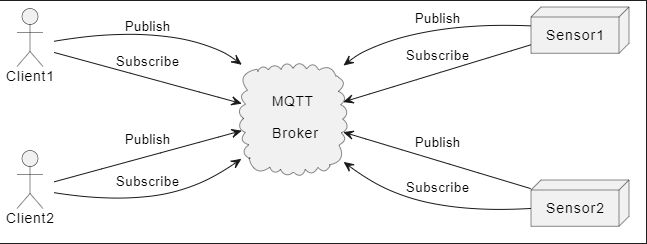
\includegraphics[scale=0.8]{figs/MQTTBrokerArchitecture.png}
    \caption{Arhitectura publica/aboneaza a protocolului MQTT}
    \label{fig:MQTTBrokerArchitecture}
\end{figure}

Subeictul mesajelor, denumit topic in standard [1], reprezinta o serie de cuvinte structurate pe nivele care descriu intr-un mod succint datele mesajului. 
Aceste cuvinte sunt separate prin caracterul special "/", denumit si separator de nivel [1], si au rolul de a filtra mesajele trimise catre clienti. 
De exemplu, Un senzor transmite un mesaj care contine date de temperatura catre Broker sub subiectul "IDsenzor/citiri/temperatura". 
Broker-ul va redirectiona acest mesaj doar catre clientii care sunt abonati pentru receptia de mesaje care au subiectul "IDsenzor/citiri/temperatura".

Structura unui mesaj MQTT este de tip binar, fiecare bit sau grupare de biti indentifica un tip de mesaj sau diferite proprietati, in comparatie cu alte 
protocoale de comunicatie care utilizeaza un format bazat pe text, unde tipurile de mesaje sau proprietatile sunt identificate prin text, de exemplu,
protocolul de comunicatie HTTP. Principalul avantaj al formatului de tip binar este dimensiunea scazuta a pachetului. Tabelul \ref{tab:StructuraMesajMQTT} 
contine o prezentare generala a acestui pachet unde:
\begin{itemize}
	\item Control Field - reprezinta octetul de control al pachetului si este impartit in doua zone:
    \begin{itemize}
        \item Tipul pachetului in primii 4 biti
        \item Semnale pentru activarea sau dezactivarea unor proprietati
    \end{itemize}
	\item Remaining Length - poate avea o lungime cuprinsa intre 1 si 4 octeti si reprezinta lungimea ramasa in pachet, adica lungimea campurilor Variable Header 
    si Payload
	\item Variable Header - are o lungime variabila care este cuprinsa in campul precedent. Acest camp difera in functie de tipul mesajului, de exemplu, in 
	cazul mesajului de publicare a datelor acest camp contine subiectul.
	\item Payload - are o lungime variabila care este cuprinsa in campul Remaining Length si reprezinta partea utila a mesajului, de exemplu, datele citite de 
	la senzor.
\end{itemize}

\begin{table}[ht]
    \caption{Structura mesaj MQTT}
    \centering                          % tabel centrat
    \begin{tabular}{|c|c|c|c|}          % 4 coloane centrate
        \hline
        1 B & 1-4 B & x B & x B \\ [0.5ex]   % inserare tabel
        %heading
        \hline                              % linie orizontal simpla
        Control Field & Remaining Length & Variable Header & Payload \\               % corpul tabelului
        \hline
    \end{tabular}
    % titlul tabelului
    \label{tab:StructuraMesajMQTT}                % eticheta folosita pentru referirea tabelului in text; referirea in text se va face cu \ref{table:nonlin}
\end{table}

Tranzactia reprezinta un schimb de mesaje intre un client si Broker si are o structura de tip cerere si confirmare. Cererea este un mesaj care contine informatii 
utile, de exemplu, datele unui senzor sau datele necesare conectarii la Broker, iar confirmarea este un mesaj prin care Borker-ul instiinteaza clientul ca cererea 
lui a fost inregistrata. Acestea din urma sunt transmise si in caz de eroare si in caz de success, iar acest lucru este semnalat in campul "Variable Header" 
prezentat in tabelul \ref{tab:StructuraMesajMQTT}. Protocolul MQTT contine mai multe tipuri de mesaje impartite pe cele doua categorii prezentate mai sus dintre 
care cele mai importante sunt prezentate in cele ce urmeaza:
\begin{itemize}
    \item CONNECT - acest pachet este trimis de catre client pentru a realiza o conexiune cu Broker-ul.
    \item CONNACK - acest pachet este trimis de catre Broker si reprezinta raspunsul pentru mesajul CONNECT si are rolul de a confirma realizarea conexiunii.
    \item PUBLISH - acest pachet este trimis de catre client si contine subiectul si datele utile.
    \item PUBACK - acest pachet este trimis de catre Broker ca raspuns la mesajul PUBLISH.
    \item SUBSCRIBE - acest pachet este trimis de catre client si reprezinta cererea de abonare la un anumit subiect. Subiectul este continut in pachet.
    \item SUBACK - acest pachet este trimis de catre Broker si reprezinta confirmarea subscriptiei clientului.
\end{itemize}

Conexiunea dintre client si Broker se realizeaza la cererea clientului print trimiterea unui mesaj specific. Acest tip de mesaj contine un camp special 
denumit "keep alive" prin care clientul informeaza Broker-ul de durata de viata a conexiunii dintre acestia. Clientul poate alege inchiderea conexiunii 
cu Broker-ul dupa fiecare mesaj de publicare a datelor cu scopul de a intra intr-un mod de consum de putere redus pana la urmatoarea perioada de 
publicare. Salvarea energiei aduce cu sine cresterea numarului de mesaje interschimbate intre client si Broker, dar aduce avantaje in durata de viata 
a bateriei. 

\subsection{Wi-Fi}\label{sec:wifi}
\subsection{SPI}\label{sec:spi}
\subsection{I2C}\label{sec:i2c}
\section{Modele abstracte}\label{sec:modele}
\subsection{RESTful API utilizand framework-ul Flask}\label{sec:flask}
RESTful API vine de la Representational State Transfer Appication Programming Interface si reprezinta un set de reguli care trebuie respectate in construirea 
unei arhitecturi web pentru a beneficia de cerinte non-functionale precum, un grad mare de scalabilitate, reliabilitate si adaptabilitate. 
Acest set de reguli are ca scop decuplarea in grad cat mai mare a clientului de sarcinile serverului.

Framework-ul Flask este o arhitectura software de module reutilizabile care are scopul de a automatiza si standardiza modul in care sunt scrise aplicatiile 
web. Acesta este scris in limbajul de programare Python si este denumit micro-framework, deoarece are o complexitate redusa si nu necesita biblioteci externe 
pentru functionalitatile comune unei apicatii web, cum ar fi operatiile pe o baza de date.

In paragrafele urmatoare se vor detalia caracteristicile cheie ale standardului arhitectural RESTful si ale framework-ului Flask.



\subsection{Retrofit}\label{sec:retrofit}
\section{IoT}\label{sec:iot}
\section{Distributed System}\label{sec:distributed}
\section{Zynq or Microprocessor architecture}\label{sec:zynq}
\section{C embedded modularization}\label{sec:cembedded}
\section{Data visualisation algorithms}\label{sec:graph}
\section{Baza de date MongoDB}\label{sec:mongodb}
MongoDB este o baza de date orientata pe documente fiind printre putinele baze de date diferita de cele uzuale care sunt relationale, adica stocheaza datele in tabele 
grupate intre ele prin relatii. Aceasta baza de date stocheaza datele in colectii de documente, de aici si denumirea de baza de date orientata pe documente. 
Structura acestui tip de baze de date permite un grad inalt de scalabilitate prin impartirea si distribuirea unei baze de date foarte mari pe mai multe 
servere. In paragrafele care urmeaza vor fi descrise caracteristicile cheie ale bazei de date.

Documentul reprezinta un singur set de date si poate fi asociat cu un inlocuitor al unui rand dintr-o baza de date relationala. Setul de date este stocat intr-un 
format numit BSON, Binary-JSON, care este o reprezentare in binar a formatului de fisiere JSON. Acesta din urma este un format de fisiere bazat pe text,
are o structura de tipul cheie-valoare si este usor de interpretat de catre om.

Figura \ref{fig:MongoDBDocument} prezinta structura unui document dintr-o baza de date MongoDB si, de asementea, formatul JSON.
\begin{figure}[H]
    \centering
    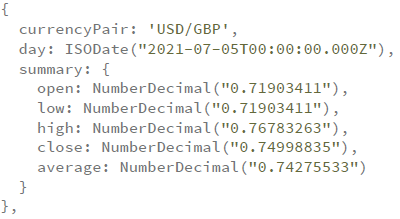
\includegraphics[scale=0.8]{figs/mongoDBDocument.png}
    \caption{Exemplu de document [2]}
    \label{fig:MongoDBDocument}
\end{figure}

Colectiile de tip serii in timp reprezinta un tip de colectii optimizate pentru a stoca si interoga documentele ordonate in timp. Aceste documente au in 
componenta un camp obligatoriu care reprezinta momentul de timp la care datele au fost achizitionate. In documentul prezentat in figura \ref{fig:MongoDBDocument} 
se poate observa perechea de valori "day" si data si ora in format ISO. Acest tip de colectii este utilizat cu preponderenta in IoT datorita faptului ca sunt 
optimizate pentru structura de date uzuala unui senzor. O astfel de structura contine, in general, un moment de timp la care achizitia de date a fost efectuata, 
un identificator unic al senzorului, in mod uzual adresa MAC, si valoarea metricii sau a metricilor achizitionate.

MongoDB creeaza automat un indice, o cheie primara, pentru fiecare document pentru a se asigura ca nu exista doua documente cu acelasi indice. In acelasi timp 
permite creearea unui indice secundar care poate contine unul sau mai multe campuri din setul de date si care are ca scop plierea pe structura fiecarui set de date 
si pe tipul de interogari cel mai des efectuate. In cazul seriilor in timp cele mai uzuale interogari sunt bazate pe timp, deci indicele ar trebui sa contina campul 
de timp la care trebuie specificata si ordonarea elementelor, de exemplu, intr-un sistem in care interogarea cea mai des intalnita este retragerea documentelor 
din ultimele 24 de ore ordonarea trebuie efectuata in ordine descrescatoare a timpului. Pe langa campul de timp, indicele mai poate contine inca un camp pentru 
a acoperi cazurile in care interogarea se face nu doar pe o perioada de timp, ci si pe o alta valoare continuta in setul de date, de exemplu, campul care contine 
adresa MAC a senzorului. MongoDB va stoca datele in functie de acest indice obtinand astfel interogari foarte eficiente. Totodata un indice prea complex sau 
scris incorect va creste complexitatea scrierii in baza de date si automat va scadea eficienta. 


{\color{blue}Împreună cu \textbf{următoarele} 2 capitole trebuie să reprezinte aproximativ 70\% din total.\\}

Scopul acestui capitol este de a explica principiile funcționale ale aplicației implementate.
Aici se va descrie soluția propusă dintr-un punct de vedere teoretic - explicați și demonstrați proprietățile și valoarea teoretică:
\begin{itemize}
	\item algoritm utilizat sau propus
	\item protocoale utilizate
	\item modele abstracte
	\item explicații/argumentări logice ale soluției alese
	\item structura logică și funcțională a aplicației.
\end{itemize}


~\\\parbox[c]{\textwidth}{\color{red}\bfseries

NU SE FAC referiri la implementarea propriu-zisă.

NU SE PUN descrieri de tehnologii preluate cu copy-paste din alte surse sau lucruri care nu țin strict de proiectul propriu-zis (materiale de umplutură).
}

\section{Nume de secțiune}\label{sec:context}

\subsection{Nume de subsecțiune}\label{subsec:numesub}

Fiecare tabel introdus în lucrare este numerotat astfel: Tabel x.y, unde x reprezintă numărul capitolului, iar y numărul tabelului din capitol.
Se lasă un rând liber între tabel și paragraful anterior, respectiv posterior (tabelul~\ref{tab:nonlin}).

\begin{table}[ht]
    \caption{Rezultate}
    \centering                          % tabel centrat
    \begin{tabular}{|c|c|c|c|}          % 4 coloane centrate
        \hline
        Case & Method\#1 & Method\#2 & Method\#3 \\ [0.5ex]   % inserare tabel
        %heading
        \hline                              % linie orizontal simpla
        1 & 50 & 837 & 970 \\               % corpul tabelului
        2 & 47 & 877 & 230 \\
        3 & 31 & 25 & 415 \\[1ex]           % [1ex] adds vertical space
        \hline
    \end{tabular}
    % titlul tabelului
    \label{tab:nonlin}                % eticheta folosita pentru referirea tabelului in text; referirea in text se va face cu \ref{table:nonlin}
\end{table}


Fiecare figură introdusă în text este citată (de ex: în figura x.y este prezentată ...) și numerotată.
Numerotarea se face astfel Figura x.y unde x reprezintă numărul capitolului iar y numărul figurii în acel capitol.
Numerotarea o face automat latex pe baza etichetei (\verb+\label{}+).

Referirea unei figuri se face cu \verb+\ref{}+. De exemplu, referința: figura~\ref{fig:imag}.

\begin{figure}[ht]
    \centering
    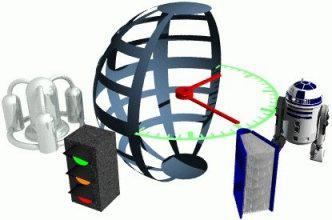
\includegraphics[]{figs/test.jpg}
    \caption{Numele figurii}
    \label{fig:imag}
\end{figure}

